\documentclass{article}

% Language setting
% Replace `english' with e.g. `spanish' to change the document language
\usepackage[english]{babel}

% Set page size and margins
% Replace `letterpaper' with`a4paper' for UK/EU standard size
\usepackage[letterpaper,top=2cm,bottom=2cm,left=3cm,right=3cm,marginparwidth=1.75cm]{geometry}

% Useful packages
\usepackage{amsmath}
\usepackage{graphicx}
\usepackage[colorlinks=true, allcolors=blue]{hyperref}

\title{Customer segmentation challenge for Analysts}
\author{Carlos Rodríguez}

\begin{document}
\maketitle

% \begin{abstract}
% Your abstract.
% \end{abstract}

\section{Introduction}

One of the most important and interesting problems that one can face in a Machine learning project is the study of the importance of different parameters when building a model. Through this work, we face this problem in a classification problem, where we try to predict if a customer will be converted or not from basic information of the customers. To approach this task, we will first look into the data and pre-process it, then the data will be inspected, by trying to find some trivial relations between the prediction and the different features; and finally, we will create two different models and test how the different features affect the accuracy of the models.

\section{Pre-processing}

The pre-processing of the data is a simple task were we will convert the data and make it a suitable as possible for the models we shall train. For this, I have decided to use the data as a \texttt{pandas} \texttt{DataFrame}, which makes it simple to visualize and work with it. This data has 10 features and 891 rows, where the only feature that is not important and we shall avoid using is the \texttt{user\_id}, as this are individual labels for each user and will only miss lead the model.

The first task is to open the dataset, which is saved in an Excell file called \texttt{Data\_Scientist\_-\_Case\_\\Dataset.xlsx}; and transform it into a \texttt{DataFrame}. Here we find some formatting issues, caused by the way the data has been saved, it is not saved into columns, but just in one column where all the features are separated by commas.

The second task is to look into empty values, as it is seen there are 2 missing values in the feature \texttt{branch} and 177 in \texttt{age}. One could decide to erase all those rows or try to give random values. For the 2 empty branches it is better to just erase them, 2 users out of 891 is not important, if they were more, we could take that as a new branch itself. For the 177 users who did not give an age, due to the lack of prior information, it was decided to be erased, giving a random value to them, as 0 or 100, or the mean of the rest of ages, could generate a bias towards this values and the model should work properly with 712 users, we are not trying to make the model as precise as possible. It is important to highlight, that the use of empty values might not be a problem for some models so one could have continue without erasing them.

The second step is to convert all the parameters with string values to numbers. Here we convert the variables \texttt{gender}, \texttt{credit\_account\_id} and \texttt{branch} to discrete numbers. The gender is changes to 0 for female and 1 for male and the branches are given the values 0 for Helsinki, 2 for Tampere and 3 for Turku. For the case of the credit account we know that those who did not share this information have the token \texttt{9b2d5b4678781e53038e91ea5324530a03f27dc1d0e5f6c9bc9d493a23be9de0}, while the other have their own personal token. Hence we separate between users who share this information, giving them the value 1, and those who did not share it, giving them the value 0.

The last step one could do is to normalize the data, but this was not done as the results would not change when normalizing. Hence, the data is cleaned and useful for the next step.

Before continuing, we have to remind that we do not have any prior information about what does convert means, we will assume that it is related to a positive aspect in the working out routine of users and their capability to engage to the app of the company, although this might bias our hypothesis, the way we look into the data and our conclusions. Still, the working process will count with the objectiveness of statistical processes and mathematical analysis, maintaining the unbiased of the raw results.


\section{Visualization}

Before creating a model it is interesting to see if we can already get some intuition of the solution. For that, we will inspect the data and the relation between single parameters and the parameter we want to predict. This is possible because the number of parameters is quite tiny, we only have 8 parameters, as the \texttt{user\_id} is already erased; and most of them are discrete.

In figure~\ref{fig:Scatter} we can see the a scatter of the different features in the file versus the classification task, \texttt{converted}. In this figure, we cannot see anything, there is no parameter that seem to be specially relevant. It is important to mention that this scattering plot is quite poor as it does not give any clue how many points we have in each category, there could be only 1 male who converted or 100, but we do not see any different. Hence, it is more interesting to look at some discrete variables and see the probability of each to convert.

To make the comparison inside features, we will choose 3 interesting categories, to simplify this task, \texttt{gender}, \texttt{customer\_segment} and \texttt{branch}. The reason for choosing this 3 parameters is that, although we do not have any prior information they seem interesting and they have between 2 and 3 different categories. Non of the variables are balanced, there is 3 times more men than women, more than half of the customers belong to the segment 13 and the rest are, more or less, evenly distributed in the other 2 segments and nearly 80~\% of the users are part of the Helsinki branch, while only 4~\% belong to Turku, and the remaining to Tampere. This might create some bias when categorizing.

\begin{table}[!h]
\begin{center}
\begin{tabular}{ c | c  c | c c c | c c c}
  & female & male & 11 & 12 & 13 & Helsinki & Tampere & Turku \\
 Converted & 63.6~\% & 75.3~\% &  65.2~\% & 48~\% & 23.9~\% & 36.3~\% & 60.8~\% & 28.6~\%
\end{tabular}
\caption{\label{tab:perc}Percentage of converted users in each category}
\end{center}
\end{table}

As seen in table~\ref{tab:perc}, males tend to get converted a 10~\% more, the segment 11 is more probable to convert than segments 12 and 13 by around 15~\% and 40~\% respectively and if you are from Tampere, your probabilities of converting are nearly 35~\% higher than if you are from Helsinki and around 30~\% higher than if you are from Turku. Hence, we can see a pattern here, this features might be really important when trying to predict if a user will convert. Now, we have to test this features.


\begin{figure}
\centering
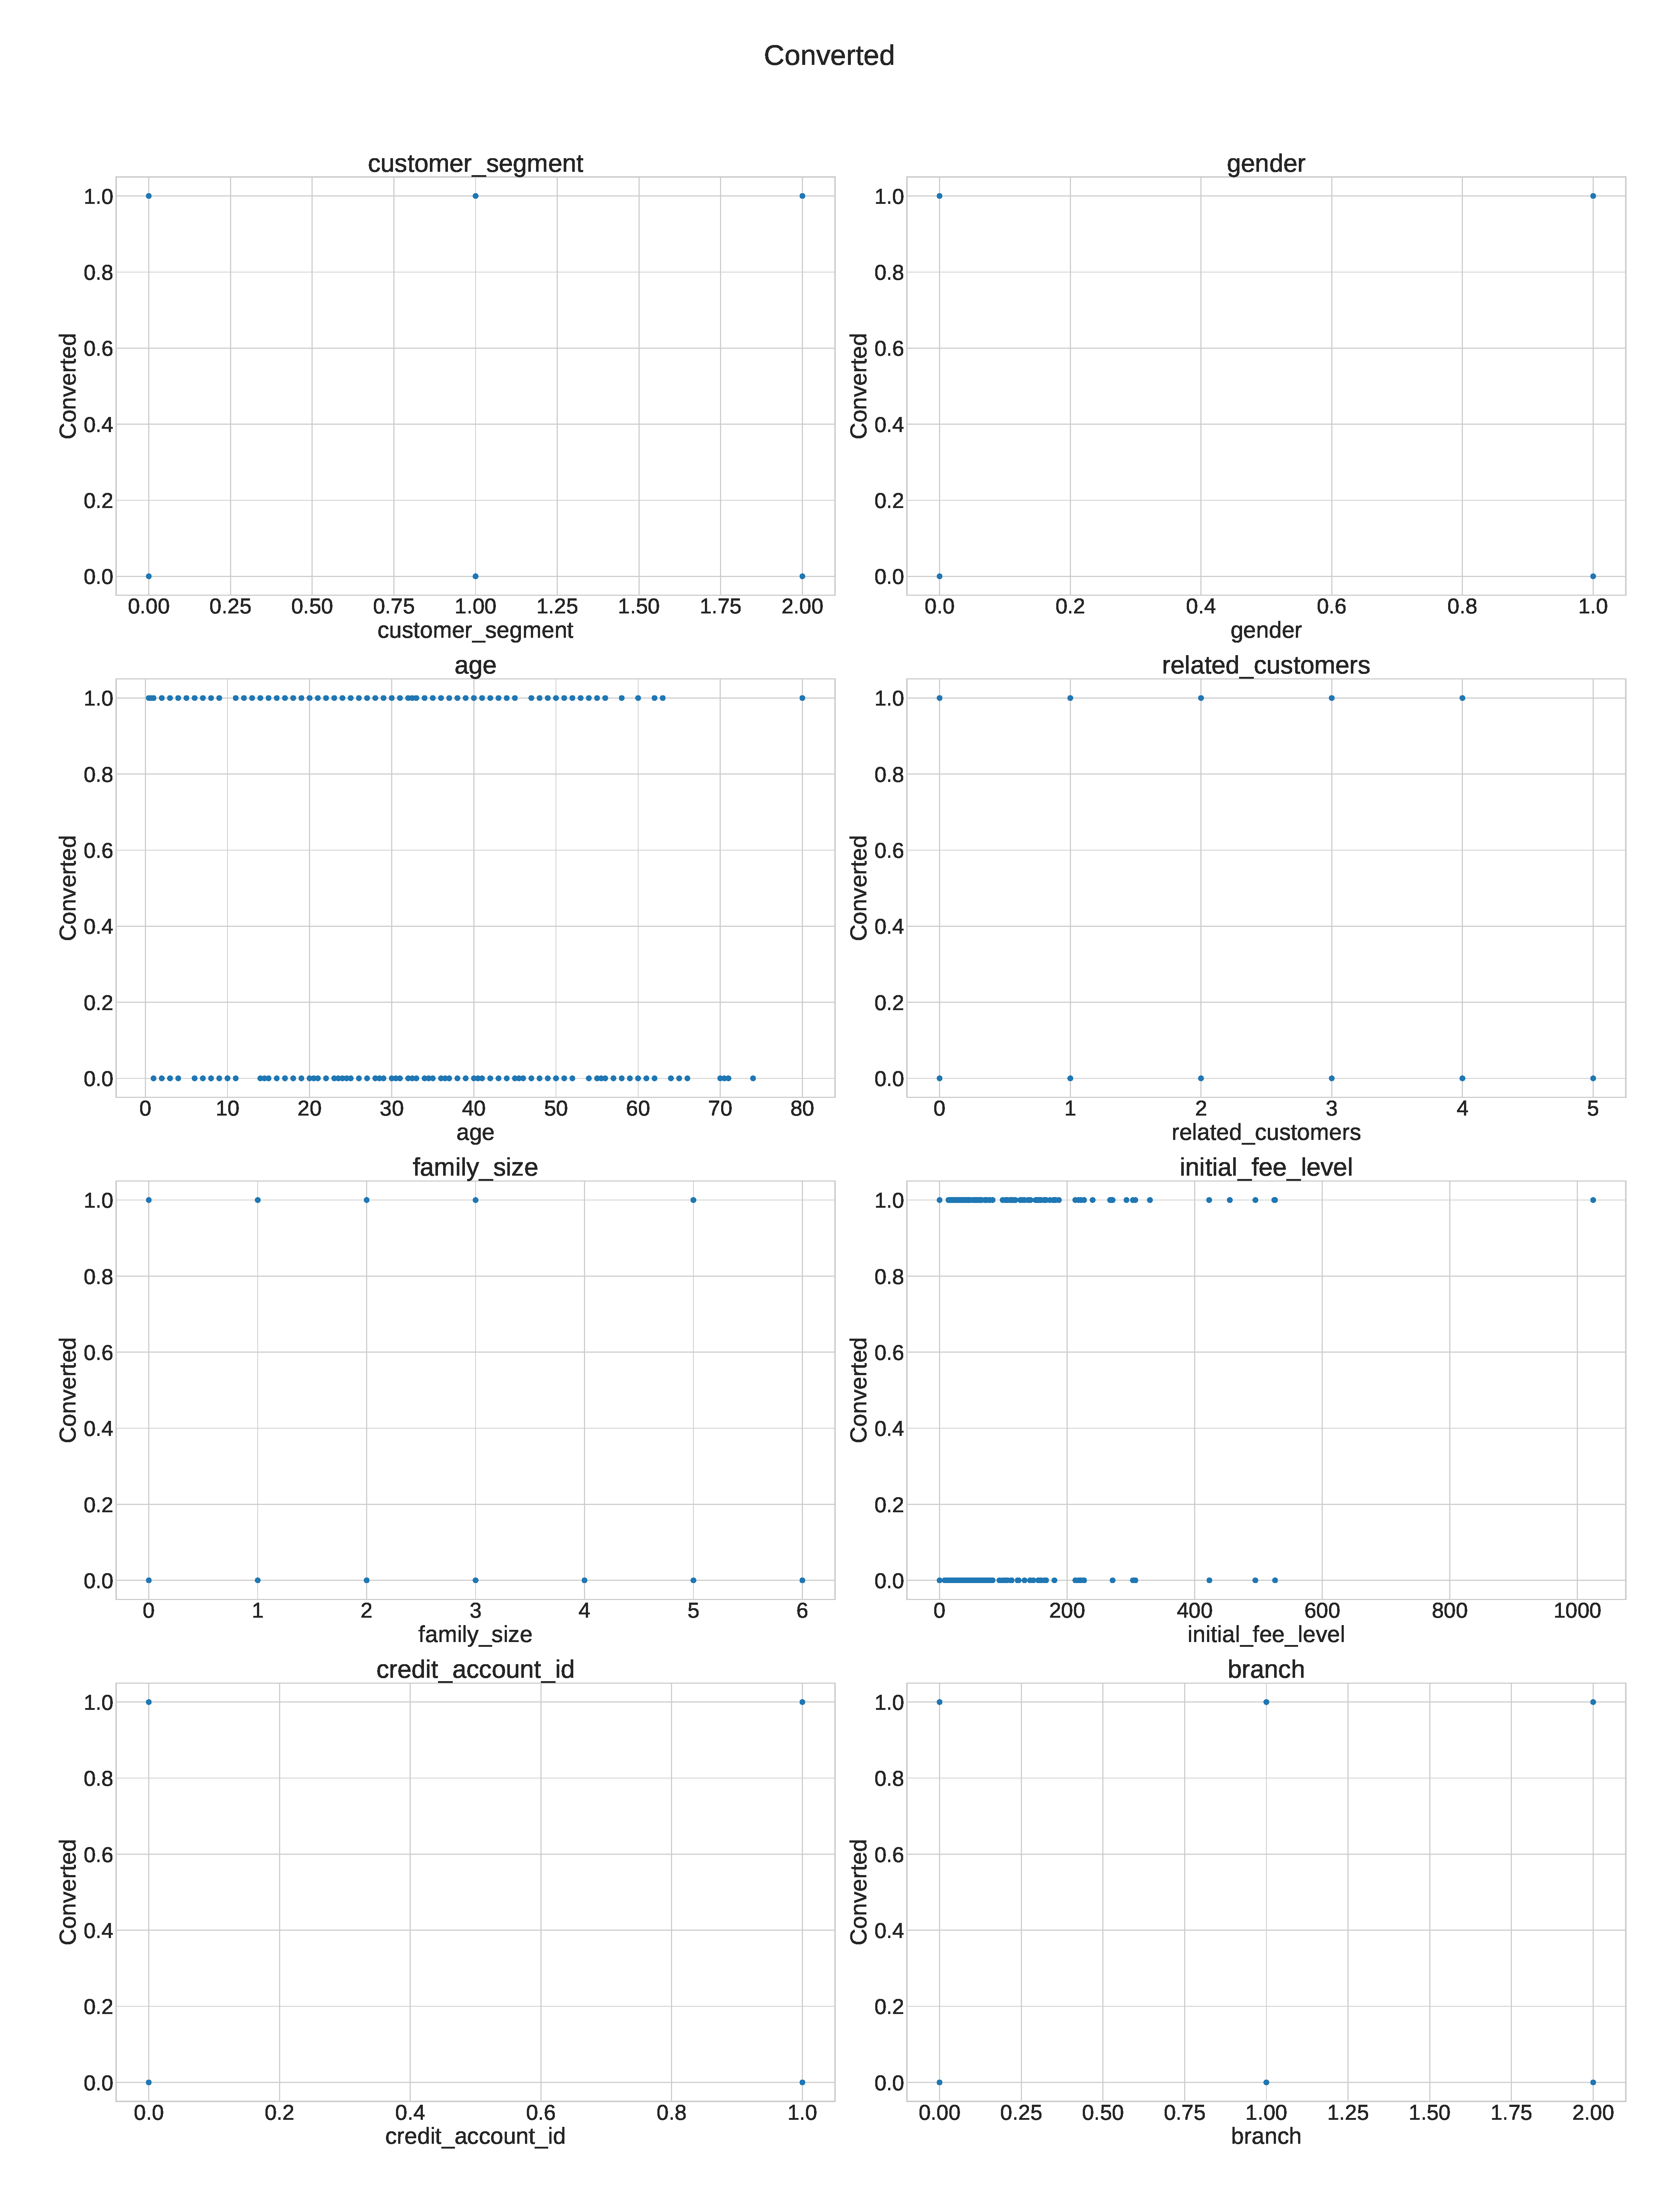
\includegraphics[width=1\textwidth]{Figures/Scatter.pdf}
\caption{\label{fig:Scatter}Plots of the converted parameter against all the other parameters, from top to bottom and left to right, \texttt{customer\_segment}, \texttt{gender}, \texttt{age}, \texttt{related\_customers}, \texttt{family\_size}, \texttt{initial\_fee\_level}, \texttt{credit\_account\_id} and \texttt{branch}.}
\end{figure}

\section{Modelling}

Finally, after having an idea of the data set, we will test how do the variable perform when they are given to a model, we want to find the most relevant parameters when predicting if a user will convert or not. for this propose, we are going to create 2 classification models, we want to check if they agree, and we will measure the accuracy of the models. Them, we will use the \texttt{permutation\_importance} function from \texttt{scikit-learn} to check which parameters are more relevant for this task. This function tries the prediction capabilities of the models when the different parameters are omitted, allowing us to calculate the importance of each parameter, which is the reduction of in the prediction in the model.

First, we shall separate the data in a training set and a validation set in a 75:25 ratio. Second, we create an \texttt{AdaBoostClassifier} and a \texttt{XGBClassifier} models and we fit them with the training set. Finally, we apply the \texttt{permutation\_importance} function with the validation set to measure the importance. The result can be seen in figure~\ref{fig:featur}, where we can see that \texttt{gender} is the most important feature by far, followed by \texttt{age} and \texttt{customer\_segment}. the solution seem quite consistent between both models although \texttt{customer\_segment} seem to be 5~\% more important for the XGBoost model and the features \texttt{related\_customers} and \texttt{initial\_fee\_level} seem to fight for the position of fourth most important features. from the rest, \texttt{family\_size} and \texttt{credit\_account\_id} are completely irrelevant in both cases.


\begin{figure}
\centering
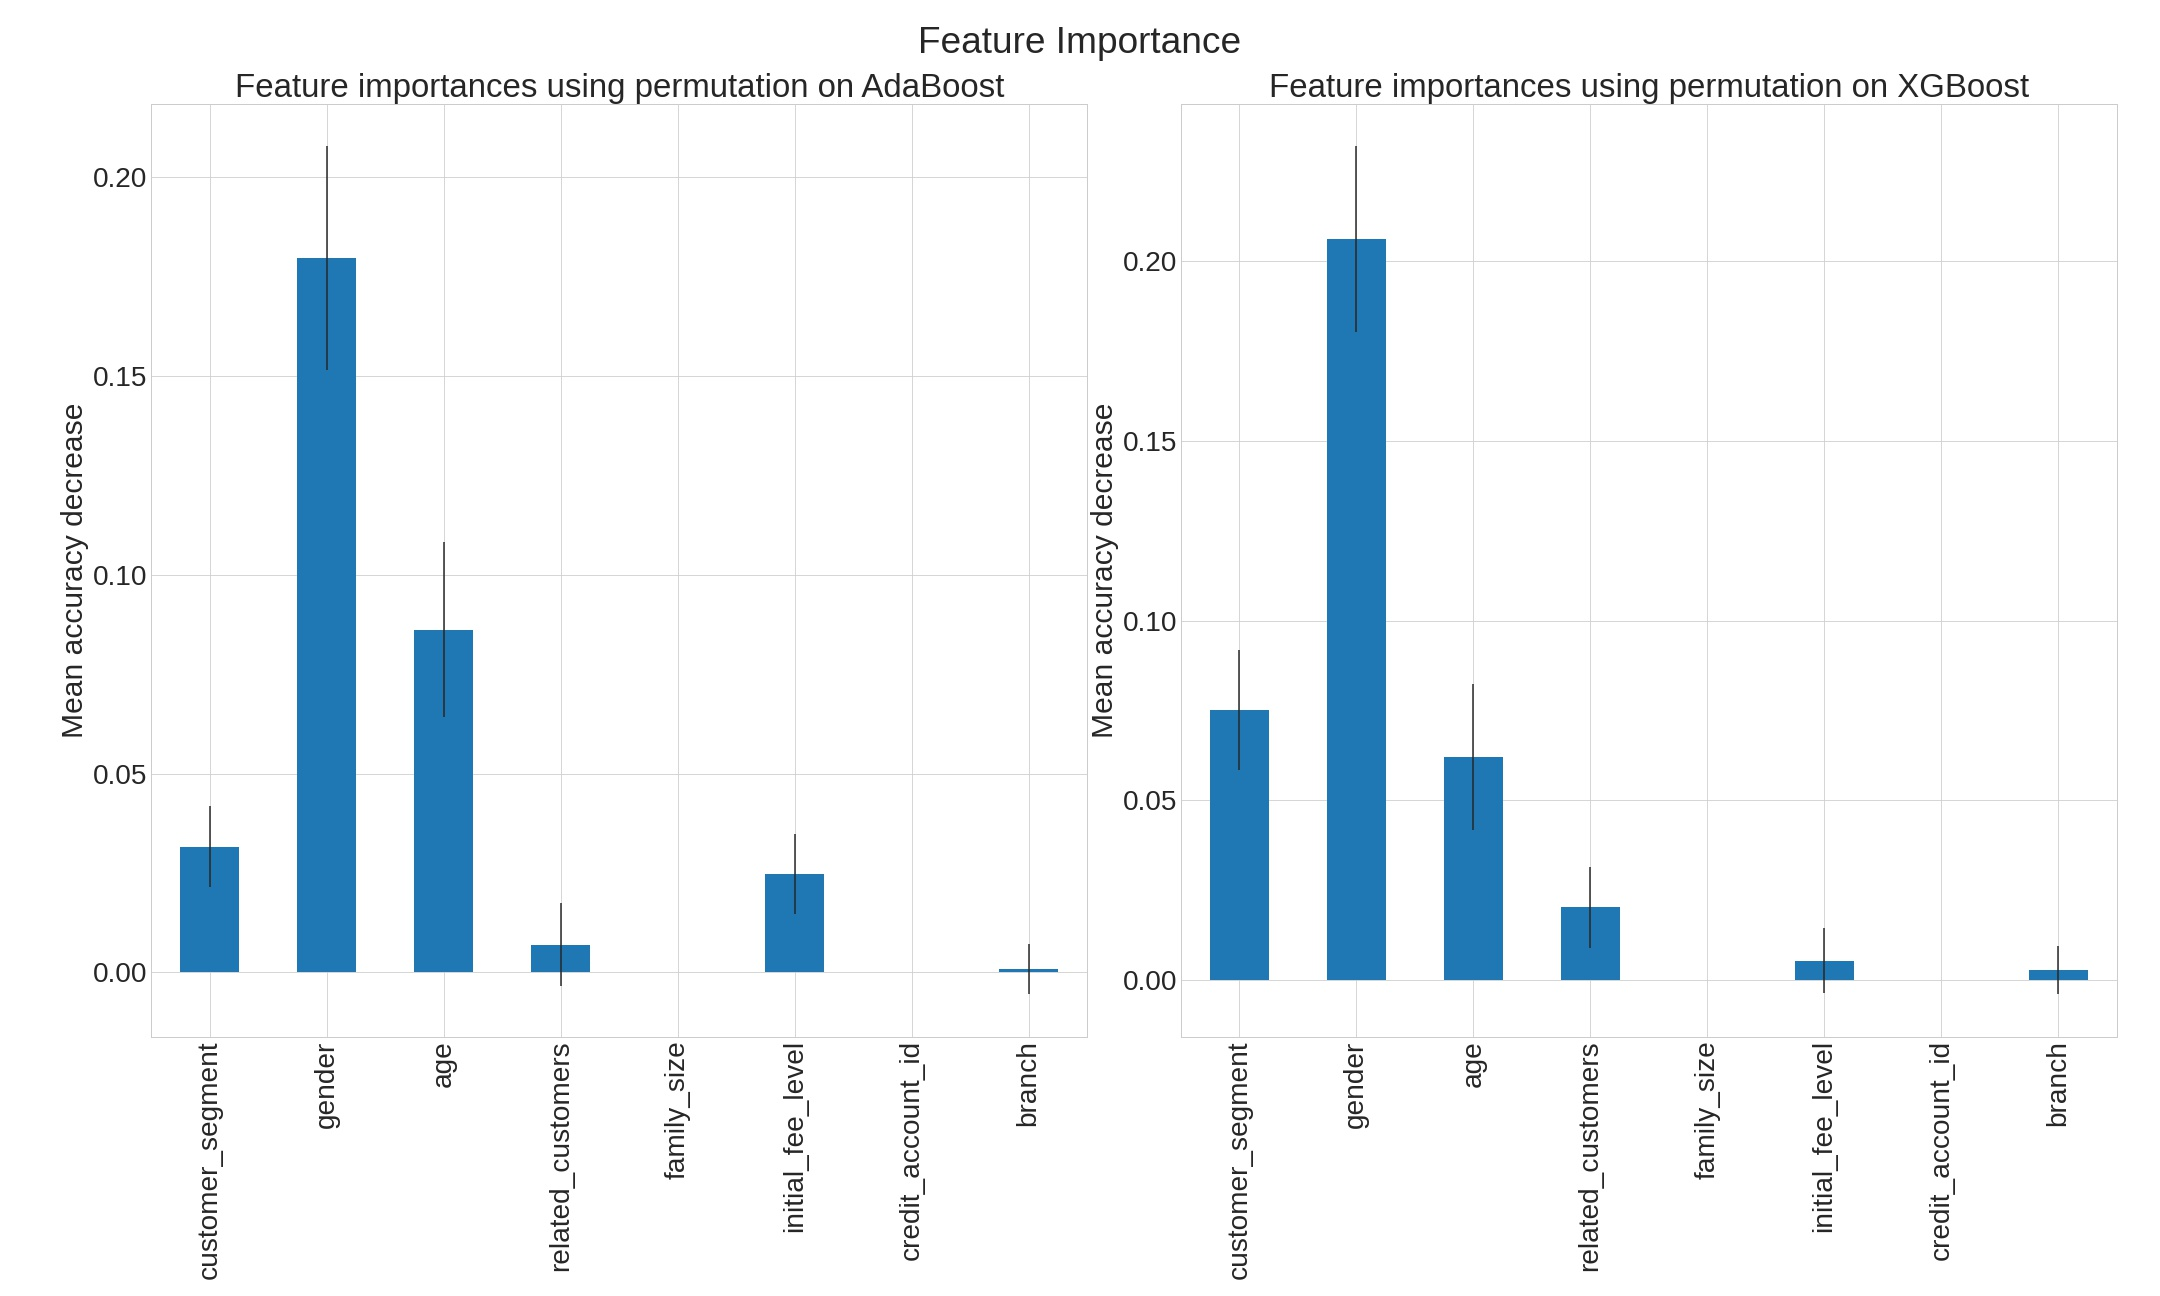
\includegraphics[width=1\textwidth]{Figures/Feature_importance.jpeg}
\caption{\label{fig:feature}Plots of the importance for the different parameter. The plots are separated in 2, one per model, the \texttt{AdaBoostClassifier} in the left and \texttt{XGBClassifier} in the right}
\end{figure}



\section{Conclusions}

To conclude we can accept that the 3 more important features for this classification task are \texttt{gender}, \texttt{age} and \texttt{customer\_segment}, highlighting \texttt{gender}. However, the parameters \texttt{related\_costumers}, \texttt{initial\_fee\_level} and \texttt{branch} are still important and the last two parameters \texttt{family\_size} and \texttt{credit\_account\_id} are completely irrelevant.

From the parameters that are not so important, it is interesting to highlight two, \texttt{branch} and \texttt{family\_size}. Both of them seem to be neglectable, still there are arguments for them to be relevant. \texttt{family\_size} might affect the amount of free time a customer has and hence the engage to their training and the app. Same happens to \texttt{branch}, a parameter that seemed to be really important by itself, people convert much more in Tampere that in any other branch, but yet \texttt{branch} is not a decisive parameter. In the case of \texttt{branch}, when we looked at the branches, Tampere has 30 \% more probabilities of converting than in any other branch. The reason for this is more obvious than for \texttt{family\_size}, the branches are really bias Helsinki covers 80~\% of the users, hence the influence of this parameter is limited. Furthermore, the cultural aspect of the location of the different branches might seem really important, but all the branches belong to the same country, Finland. Hence, either it is just a coincidence that people in Tampere convert more or we need more data from Tampere to get a reliable correlation. For \texttt{family\_size} in general will only be significant in case it refers to number of children, as they are the ones that need more attention. However, as children grow their needs decreases and as far as you schedule yourself along with your children, you can always find time to do sport, or even do sport with your family, erasing the significance of this parameter. This lack of relevance of \texttt{family\_size} might be also related to the fact that our hypothesis of what is the \texttt{converted} parameter might be wrong

Finally, it is interesting to keep in mind that \texttt{gender} is by far the most relevant parameter. If we accept that \texttt{converted} is not a gender related variable, this result demonstrates that gender roles are still a key part of our societies and that gender keeps clustering individuals in different segments. Continuing with the hypothesis that our classification parameter is related to a positive engage with the app, this information may be useful in the way on how trigger costumers with gender specific advertisement. However this is just speculation and we already knew that men convert 10~\% more than men.


\end{document}
